\chapter{MÔ HÌNH HÓA TOÁN HỌC HỆ THỐNG}
    \section{Giới thiệu}
        \hspace*{0.6cm}Động học của robot được mô tả bởi mô hình toán học nhằm giúp cho việc phát triển hệ thống điều khiển dễ dàng hơn cho robot cân bằng. Trong phần này, các phương trình chuyển động của xe hai bánh được đưa ra chi tiết.
    \section{Các ký hiệu sử dụng}
        \begin{table}[H]
            \centering
            \begin{tabular}{|c|c|}
                \hline
                \textbf{Ký hiệu} & \textbf{Đại lượng} \\ \hline
                $x$ & Độ dịch chuyển (m) \\ \hline
                $\dot{x}$ & Tốc độ dịch chuyển (m/s) \\ \hline
                $\theta$ & Góc nghiêng (rad) \\ \hline
                $\dot{\theta}$ & Tốc độ góc (rad/s) \\ \hline
                $V_a$ & Điện áp (V) \\ \hline
                $k_m$ & Hằng số moment quay động cơ \\ \hline
                $k_e$ & Hằng số sức phản điện động \\ \hline
                $R$ & Điện trở danh định \\ \hline
                $l$ & Khoảng cách giữa trọng tâm bánh xe và trọng tâm robot \\ \hline
                $g$ & Gia tốc trọng trường \\ \hline
                $M_p$ & Khối lượng khung \\ \hline
                $r$ & Bán kính bánh xe \\ \hline
                $I_p$ & Momen quán tính của khung \\ \hline
                $I_w$ & Momen quán tính của bánh xe \\ \hline
                $M_w$ & Khối lượng của bánh xe kết nối với hai phía của robot \\ \hline
            \end{tabular}
            \caption{Bảng ký hiệu và đại lượng}
        \end{table}
    \section{Mô hình động lực học}
    \subsection*{Động năng}
    \subsubsection*{Bánh xe}
        \begin{figure}[H]
            \centering
            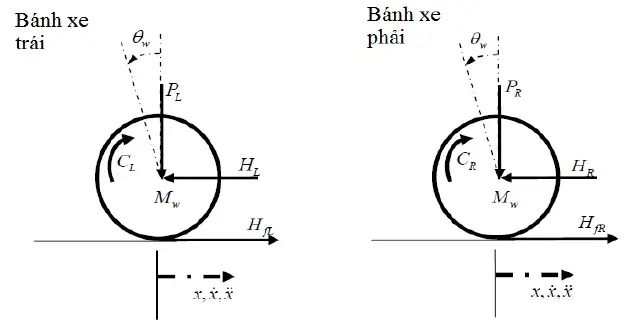
\includegraphics[width=1\textwidth]{pictures/wheel.png} 
            \caption{Sơ đồ tự do của các bánh}
        \end{figure}
        
        Động năng tịnh tiến của 1 bánh xe
        \begin{align}
            K_{w1} = \frac{1}{2} M_w \dot{x}^2
        \end{align}
        
        Động năng quay của 1 bánh xe
        \begin{align}
            K_{w2} = \frac{1}{2} I_w \omega^2 = \dfrac{1}{2} I_w \frac{\dot{x}^2}{r^2}
        \end{align}

        Tổng động năng do chuyển động của 2 bánh xe
        \begin{align}
            K_w &= 2 \cdot \left(K_{w1} + K_{w2}\right) \nonumber\\
                &= M_w \dot{x}^2 + \dfrac{I_w}{r^2} \dot{x}^2
        \end{align}
        

        
        
    \subsubsection*{Khung xe (mô hình con lắc)}
        \hspace*{0.6cm}Cấu hình robot có thể được mô hình như một con lắc ngược
            \begin{figure}[H]
                \centering
                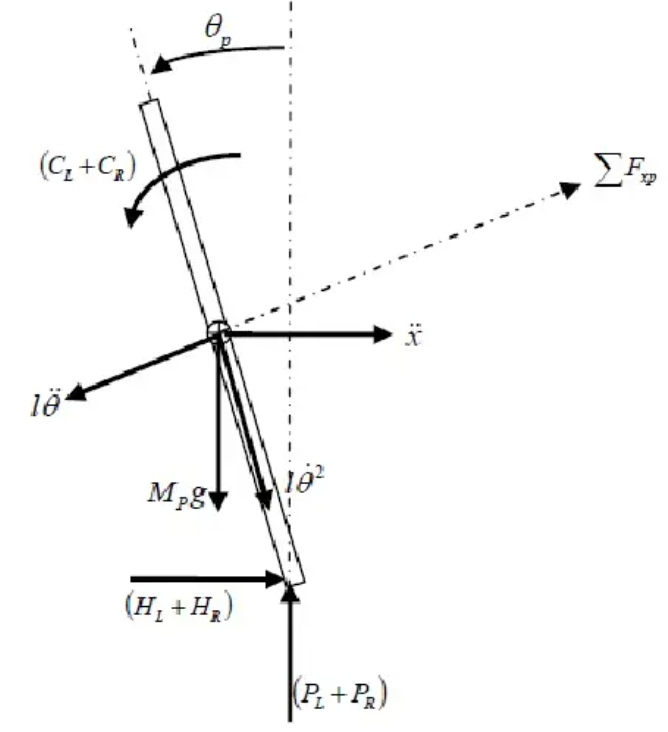
\includegraphics[width=0.5\textwidth]{pictures/inverted_pendulum.png} 
                \caption{Sơ đồ tự do của con lắc ngược}
            \end{figure}
            
            Động năng quay của khung xe
            \begin{align}
                K_{p1} = \dfrac{1}{2} I_p \dot{\theta}^2 
            \end{align}
            
            Động năng tịnh tiến của khung xe
            \begin{align}
                K_{p2} = \dfrac{1}{2} M_p v_c^2
            \end{align}
            
            Chọn gốc tọa độ tại ví trí tâm bánh xe, tọa độ khối tâm của con lắc là

            \begin{align}
                (x_c, y_c) = (x+\ell \sin(\theta), \ell \cos \theta) 
            \end{align}
            
            Vận tốc khối tâm của khung xe
            \begin{align}
                (V_{cx}, v_{cy}) = (\dot{x}+\ell \dot{\theta} \cos(\theta), -\ell \dot{\theta}\sin \theta) 
            \end{align}

            Động năng tịnh tiến của khung xe
            \begin{align}
                K_{p2} &= \dfrac{1}{2} M_p \left[(\dot{x}+\ell \dot{\theta} \cos(\theta))^2 + (-\ell \dot{\theta}\sin \theta)^2\right] \nonumber\\
                       &=\dfrac{1}{2} M_p \left[\dot{x}^2 + 2 \ell \dot{x} \dot{\theta} \cos \theta + \ell^2 \dot{\theta}^2\right] 
            \end{align}
            
            Tổng động năng của khung xe
            
            \begin{align}
                K_{p} = K_{p1} + K_{p2} = \dfrac{1}{2} I_p \dot{\theta}^2 + \dfrac{1}{2} M_p \left[\dot{x}^2 + 2 \ell \dot{x} \dot{\theta} \cos \theta + \ell^2 \dot{\theta}^2\right]
            \end{align}

            Do đó tổng động năng của hệ là
            \begin{align}
                K = K_w + K_p &= M_w \dot{x}^2 + \dfrac{I_w}{r^2} \dot{x}^2 + \dfrac{1}{2} I_p \dot{\theta}^2 + \dfrac{1}{2} M_p \left[\dot{x}^2 + 2 \ell \dot{x} \dot{\theta} \cos \theta + \ell^2 \dot{\theta}^2\right] \nonumber\\
                    &= \dfrac{1}{2} \left(2M_w + 2 \dfrac{I_w}{r^2} + M_p\right) \dot{x}^2 + \dfrac{1}{2} \left(M_p \ell^2 + I_p\right)\dot{\theta}^2 + M_p \ell \dot{x} \dot{\theta} \cos \theta \nonumber\\
                    &= \dfrac{1}{2} M_{\Sigma} \dot{x}^2 + \dfrac{1}{2} J \dot{\theta}^2 + M_p \ell \dot{x} \dot{\theta} \cos \theta
             \end{align}
             Với
             \begin{align}
                M_{\Sigma} &= 2M_w + 2 \dfrac{I_w}{r^2} + M_p \nonumber\\
                J &= M_p \ell^2 + I_p \nonumber
             \end{align}
    \subsection*{Thế năng}
            Thế năng của hệ khi khung xe nghiêng một góc $\theta_p$ so với phương thẳng đứng là:
            \begin{align}
                V = M_p g \ell \cos \theta
            \end{align}         


    \subsection*{Phương trình Lagrange}
            Phương trình Lagrange tổng quát cho cơ hệ
            \begin{align}
                \frac{d}{dt} \left( \frac{\partial L}{\partial \dot{q_i}} \right) - \frac{\partial L}{\partial q_i} = Q_i
            \end{align}

            Trong đó
            \begin{itemize}
                \item $L = K - V$: hàm Lagrange
                \item $q_i$: tọa độ suy rộng, trong phạm vi bài báo cáo ta có $q = [x \,\, \theta]^T$
                \item $\dot{q_i}$: đạo hàm theo thời gian của $q_i$
                \item $Q_i$: moment hoặc lực tổng quát (nếu có). Trong phạm vi bài báo cáo ta có $Q_i = [F_x \,\, \tau_\theta]$.
            \end{itemize}

            Hàm Lagrange
            \begin{align}
                L = K - V = \dfrac{1}{2} M_{\Sigma} \dot{x}^2 + \dfrac{1}{2} J \dot{\theta}^2 + M_p \ell \dot{x} \dot{\theta} \cos \theta - M_p g \ell \cos \theta 
            \end{align}    

            Đối với tọa độ suy rộng $x$:
            \begin{align*}
                &\frac{\partial L}{\partial \dot{x}} = M_{\Sigma} \dot{x} + M_p \ell \dot{\theta} \cos \theta\\
                &\frac{d}{dt} \left( \frac{\partial L}{\partial \dot{x}} \right) = M_{\Sigma} \ddot{x} + M_p \ell \ddot{\theta} \cos \theta - M_p \ell \dot{\theta}^2 \sin \theta\\
                &\frac{\partial L}{\partial x} = 0
            \end{align*}

            Do đó
            \begin{align}
                M_{\Sigma} \ddot{x} + M_p \ell \ddot{\theta} \cos \theta - M_p \ell \dot{\theta}^2 \sin \theta = F_x
            \end{align}


            Đối với tọa độ suy rộng $\theta$:
            \begin{align*}
                &\frac{\partial L}{\partial \dot{\theta}} = J \dot{\theta} + M_p \ell \dot{x} \cos \theta\\
                &\frac{d}{dt} \left( \frac{\partial L}{\partial \dot{\theta}} \right) = J \ddot{\theta} + M_p \ell \ddot{x} \cos \theta - M_p \ell \dot{x} \dot{\theta} \sin \theta\\
                &\frac{\partial L}{\partial \theta} = -M_p \ell \dot{x} \dot{\theta} \sin \theta - M_p g \ell (-\sin \theta) = -M_p \ell \dot{x} \dot{\theta} \sin \theta + M_p g \ell \sin \theta
            \end{align*}

            Do đó
            \begin{align}
                J \ddot{\theta} + M_p \ell \ddot{x} \cos \theta - M_p \ell \dot{x} \dot{\theta} \sin \theta + M_p \ell \dot{x} \dot{\theta} \sin \theta - M_p g \ell \sin \theta = \tau_\theta \nonumber\\
                \Leftrightarrow J \ddot{\theta} + M_p \ell \ddot{x} \cos \theta - M_p g \ell \sin \theta = \tau_\theta
            \end{align}

            Từ phương trình (1.13) và (1.15) ta có hệ 

            \begin{equation}
                \begin{cases}
                    M_{\Sigma} \ddot{x} + M_p \ell \ddot{\theta} \cos \theta - M_p \ell \dot{\theta}^2 \sin \theta = F_x \\
                    J \ddot{\theta} + M_p \ell \ddot{x} \cos \theta - M_p g \ell \sin \theta = \tau_\theta
                \end{cases}
            \end{equation}

        
        
        Trong chương tiếp theo, ta sẽ tiến hành thiết kế và mô phỏng các bộ điều khiển dựa trên hàm truyền đã thu được.
            
        
       